Completa la tabla \ref{tab:3.11}.

\begin{table}[H]
    \rowcolors{1}{}{lightgray!20}
    \centering
    \caption{Perímetros}
    \label{tab:3.11}
    \begin{tabular}{|c|>{\centering}p{3cm}|c|p{3cm}|}
        \toprule                 \rowcolor{colorrds!80}
        \textbf{\color{white}Figura}                                     & \textbf{\color{white}Perímetro} & \textbf{\color{white}Figura}                                     & \textbf{\color{white}Perímetro} \\ \midrule
        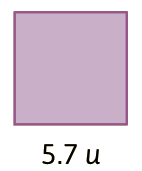
\includegraphics[width=0.1\linewidth]{../images/20230319021432}  & \ifprintanswers\fi              & 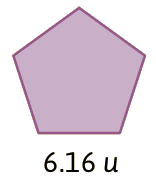
\includegraphics[width=0.13\linewidth]{../images/20230319021457} & \ifprintanswers\fi              \\ \hline
        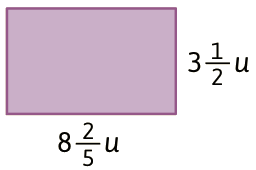
\includegraphics[width=0.18\linewidth]{../images/20230319021443} & \ifprintanswers\fi              & 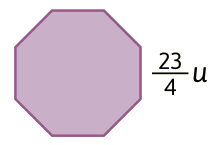
\includegraphics[width=0.16\linewidth]{../images/20230319021504} & \ifprintanswers\fi              \\ \hline
        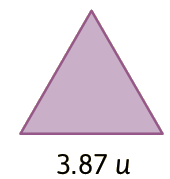
\includegraphics[width=0.14\linewidth]{../images/20230319021450} & \ifprintanswers\fi              & 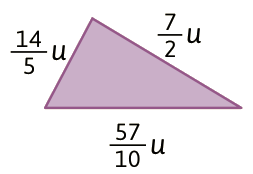
\includegraphics[width=0.18\linewidth]{../images/20230319021512} & \ifprintanswers\fi              \\ \hline
        \bottomrule
    \end{tabular}
\end{table}